\documentclass{article}
\usepackage{graphicx}
\usepackage{listings}
\usepackage{caption}
\usepackage{float}
\usepackage{amsmath}
\usepackage{amsfonts}
\usepackage{amssymb}

\title{Hospital Database Project Report}
\author{Muhammed Abdel Hamid Shelleh}
\date{\today}

\begin{document}

\maketitle

\section{Assumptions}
\begin{itemize}
    \item Each patient can only be assigned to one room at a time.
    \item Each physician and nurse have unique IDs and certification numbers.
    \item The status of health records can be either 'ongoing' or 'resolved'.
    \item Each payable is linked to an invoice.
    \item The patient balance is tracked by subtracting payments from total invoices.
\end{itemize}

\section{Enhanced Entity-Relationship Diagram (EERD)}
\begin{figure}[H]
    \centering
    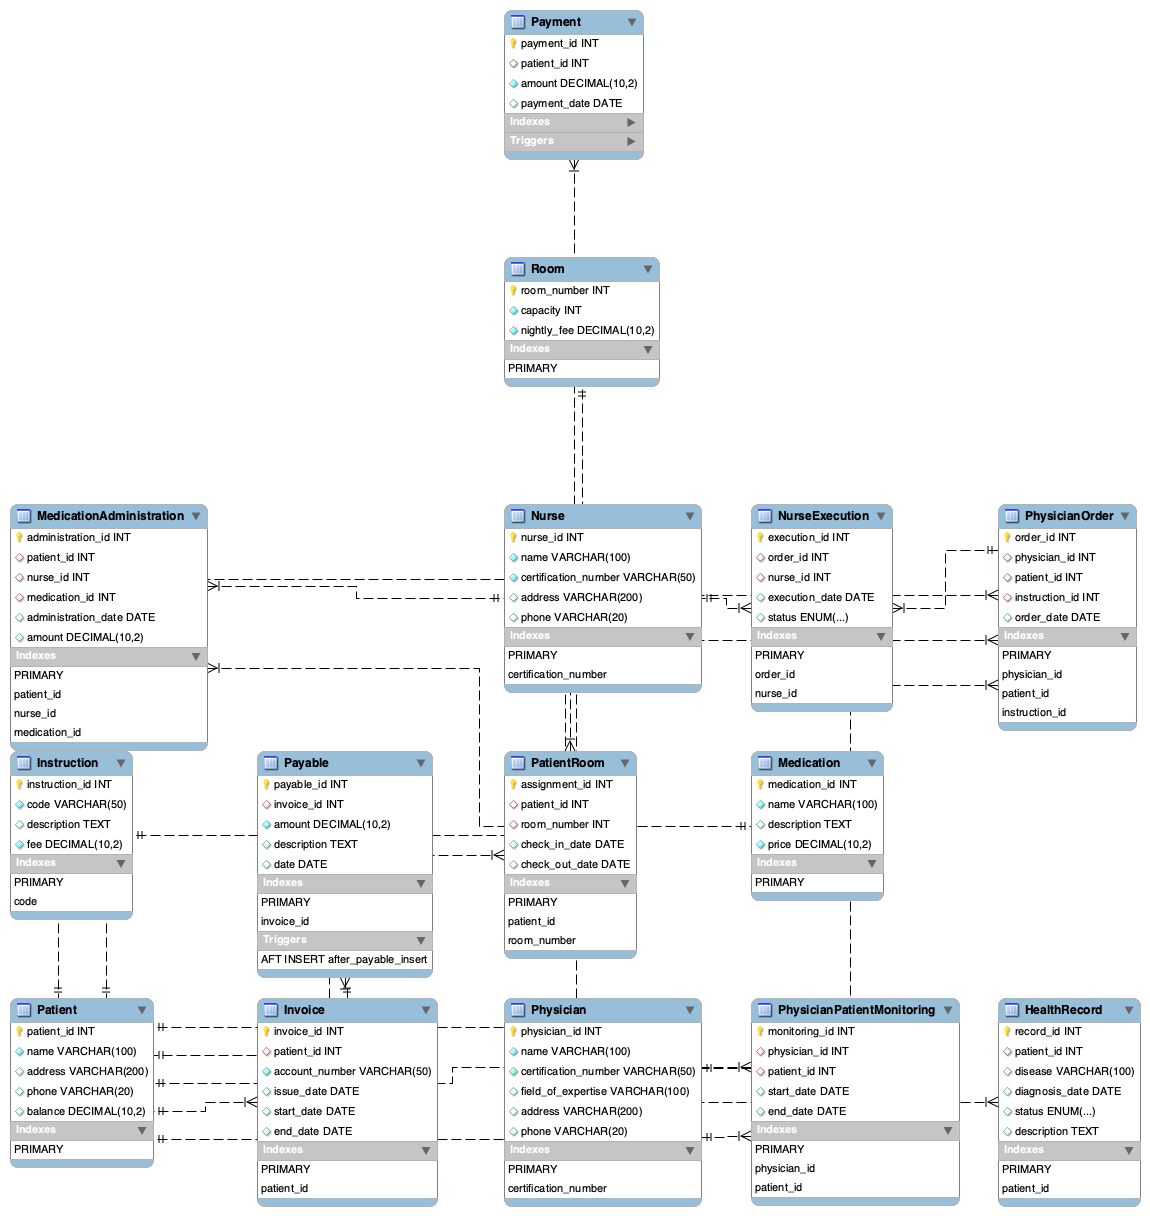
\includegraphics[width=1\textwidth]{hospital.png}
    \caption{Enhanced Entity-Relationship Diagram for the Hospital Database}
\end{figure}

\section{Relations and Keys}
\begin{itemize}
    \item \textbf{Physician(physician\_id, name, certification\_number, field\_of\_expertise, address, phone)}
        \begin{itemize}
            \item Primary Key: \{physician\_id\}
        \end{itemize}
    \item \textbf{Nurse(nurse\_id, name, certification\_number, address, phone)}
        \begin{itemize}
            \item Primary Key: \{nurse\_id\}
        \end{itemize}
    \item \textbf{Room(room\_number, capacity, nightly\_fee)}
        \begin{itemize}
            \item Primary Key: \{room\_number\}
        \end{itemize}
    \item \textbf{Patient(patient\_id, name, address, phone, balance)}
        \begin{itemize}
            \item Primary Key: \{patient\_id\}
        \end{itemize}
    \item \textbf{HealthRecord(record\_id, patient\_id, disease, diagnosis\_date, status, description)}
        \begin{itemize}
            \item Primary Key: \{record\_id\}
            \item Foreign Key: \{patient\_id\} references \textbf{Patient(patient\_id)}
        \end{itemize}
    \item \textbf{PatientRoom(assignment\_id, patient\_id, room\_number, check\_in\_date, check\_out\_date)}
        \begin{itemize}
            \item Primary Key: \{assignment\_id\}
            \item Foreign Keys: \{patient\_id\} references \textbf{Patient(patient\_id)}, \{room\_number\} references \textbf{Room(room\_number)}
        \end{itemize}
    \item \textbf{PhysicianPatientMonitoring(monitoring\_id, physician\_id, patient\_id, start\_date, end\_date)}
        \begin{itemize}
            \item Primary Key: \{monitoring\_id\}
            \item Foreign Keys: \{physician\_id\} references \textbf{Physician(physician\_id)}, \{patient\_id\} references \textbf{Patient(patient\_id)}
        \end{itemize}
    \item \textbf{Medication(medication\_id, name, description, price)}
        \begin{itemize}
            \item Primary Key: \{medication\_id\}
        \end{itemize}
    \item \textbf{MedicationAdministration(administration\_id, patient\_id, nurse\_id, medication\_id, administration\_date, amount)}
        \begin{itemize}
            \item Primary Key: \{administration\_id\}
            \item Foreign Keys: \{patient\_id\} references \textbf{Patient(patient\_id)}, \{nurse\_id\} references \textbf{Nurse(nurse\_id)}, \{medication\_id\} references \textbf{Medication(medication\_id)}
        \end{itemize}
    \item \textbf{Instruction(instruction\_id, code, description, fee)}
        \begin{itemize}
            \item Primary Key: \{instruction\_id\}
        \end{itemize}
    \item \textbf{PhysicianOrder(order\_id, physician\_id, patient\_id, instruction\_id, order\_date)}
        \begin{itemize}
            \item Primary Key: \{order\_id\}
            \item Foreign Keys: \{physician\_id\} references \textbf{Physician(physician\_id)}, \{patient\_id\} references \textbf{Patient(patient\_id)}, \{instruction\_id\} references \textbf{Instruction(instruction\_id)}
        \end{itemize}
    \item \textbf{Payable(payable\_id, invoice\_id, amount, description, date)}
        \begin{itemize}
            \item Primary Key: \{payable\_id\}
            \item Foreign Key: \{invoice\_id\} references \textbf{Invoice(invoice\_id)}
        \end{itemize}
    \item \textbf{Invoice(invoice\_id, patient\_id, account\_number, issue\_date, start\_date, end\_date)}
        \begin{itemize}
            \item Primary Key: \{invoice\_id\}
            \item Foreign Key: \{patient\_id\} references \textbf{Patient(patient\_id)}
        \end{itemize}
    \item \textbf{Payment(payment\_id, patient\_id, amount, payment\_date)}
        \begin{itemize}
            \item Primary Key: \{payment\_id\}
            \item Foreign Key: \{patient\_id\} references \textbf{Patient(patient\_id)}
        \end{itemize}
\end{itemize}

\section{Views and Descriptions}
\subsection{View: Patient Billing}
\begin{lstlisting}[language=SQL]
CREATE VIEW PatientBilling AS
SELECT 
    p.name AS patient_name,
    inv.invoice_id,
    inv.issue_date,
    inv.start_date,
    inv.end_date,
    pay.amount AS payable_amount,
    pay.description AS payable_description,
    pay.date AS payable_date,
    (SELECT SUM(amount) FROM Payment WHERE patient_id = p.patient_id) AS total_payments
FROM 
    Patient p
JOIN Invoice inv ON p.patient_id = inv.patient_id
JOIN Payable pay ON inv.invoice_id = pay.invoice_id;
\end{lstlisting}
\textbf{Description}: This view provides a comprehensive billing summary for each patient, including invoice details and total payments made.

\subsection{View: Physician Performance}
\begin{lstlisting}[language=SQL]
CREATE VIEW PhysicianPerformance AS
SELECT 
    ph.name AS physician_name,
    COUNT(ppm.patient_id) AS total_patients,
    SUM(po.fee) AS total_revenue
FROM 
    Physician ph
JOIN PhysicianPatientMonitoring ppm ON ph.physician_id = ppm.physician_id
JOIN PhysicianOrder po ON ph.physician_id = po.physician_id
GROUP BY ph.name;
\end{lstlisting}
\textbf{Description}: This view evaluates physician performance by counting the number of patients monitored and calculating the total revenue generated.

\subsection{View: Room Occupancy Rate}
\begin{lstlisting}[language=SQL]
CREATE VIEW RoomOccupancyRate AS
SELECT 
    r.room_number,
    COUNT(pr.assignment_id) AS total_occupancy,
    r.capacity,
    (COUNT(pr.assignment_id) / r.capacity) * 100 AS occupancy_rate
FROM 
    Room r
JOIN PatientRoom pr ON r.room_number = pr.room_number
GROUP BY r.room_number;
\end{lstlisting}
\textbf{Description}: This view calculates the occupancy rate for each room, helping to monitor room utilization.

\section{Triggers and Descriptions}
\subsection{Trigger: After Payable Insert}
\begin{lstlisting}[language=SQL]
CREATE TRIGGER after_payable_insert
AFTER INSERT ON Payable
FOR EACH ROW
BEGIN
    UPDATE Patient
    SET balance = balance + NEW.amount
    WHERE patient_id = (SELECT patient_id FROM Invoice WHERE invoice_id = NEW.invoice_id);
END;
\end{lstlisting}
\textbf{Description}: This trigger updates the patient balance after a new payable is added, ensuring the balance reflects the latest charges.

\subsection{Trigger: After Payment Insert}
\begin{lstlisting}[language=SQL]
CREATE TRIGGER after_payment_insert
AFTER INSERT ON Payment
FOR EACH ROW
BEGIN
    UPDATE Patient
    SET balance = balance - NEW.amount
    WHERE patient_id = NEW.patient_id;
END;
\end{lstlisting}
\textbf{Description}: This trigger updates the patient balance after a payment is made, ensuring the balance reflects the latest payments.

\subsection{Trigger: Prevent Room Overbooking}
\begin{lstlisting}[language=SQL]
CREATE TRIGGER stop_overbooking
BEFORE INSERT ON PatientRoom
FOR EACH ROW
BEGIN
    DECLARE room_capacity INT;
    DECLARE current_occupancy INT;
    SET room_capacity = (SELECT capacity FROM Room WHERE room_number = NEW.room_number);
    SET current_occupancy = (SELECT COUNT(*) FROM PatientRoom WHERE room_number = NEW.room_number AND check_out_date IS NULL);
    IF current_occupancy >= room_capacity THEN
        SIGNAL SQLSTATE '45000' SET MESSAGE_TEXT = 'Room overbooking is not allowed';
    END IF;
END;
\end{lstlisting}
\textbf{Description}: This trigger prevents overbooking of rooms by checking the current occupancy before a new assignment.

\section{Queries, Descriptions, and Results}
\subsection{Query 1: Patient's Medication History}
\begin{lstlisting}[language=SQL]
SELECT 
    p.name AS patient_name,
    m.name AS medication_name,
    ma.administration_date,
    n.name AS nurse_name
FROM 
    MedicationAdministration ma
JOIN Patient p ON ma.patient_id = p.patient_id
JOIN Medication m ON ma.medication_id = m.medication_id
JOIN Nurse n ON ma.nurse_id = n.nurse_id
ORDER BY ma.administration_date;
\end{lstlisting}
\textbf{Description}: Retrieves the medication history for each patient, including the patient's name, medication name, administration date, and the nurse who administered the medication.

\subsection{Query 2: Total Medications Administered by Each Nurse}
\begin{lstlisting}[language=SQL]
SELECT 
    n.name AS nurse_name,
    COUNT(ma.administration_id) AS total_medications_administered
FROM 
    MedicationAdministration ma
JOIN Nurse n ON ma.nurse_id = n.nurse_id
GROUP BY n.name
ORDER BY total_medications_administered DESC;
\end{lstlisting}
\textbf{Description}: Counts the total number of medications administered by each nurse and orders the results from highest to lowest.

\subsection{Query 3: Patients with Above Average Payments}
\begin{lstlisting}[language=SQL]
SELECT 
    p.name,
    SUM(pay.amount) AS total_payments
FROM 
    Patient p
JOIN Payment pay ON p.patient_id = pay.patient_id
GROUP BY p.name
HAVING total_payments > (SELECT AVG(total_payments) FROM (SELECT SUM(amount) AS total_payments FROM Payment GROUP BY patient_id) AS subquery)
ORDER BY total_payments DESC;
\end{lstlisting}
\textbf{Description}: Identifies patients whose total payments are above the average payment amount.

\subsection{Query 4: Physicians with Most Patients}
\begin{lstlisting}[language=SQL]
SELECT 
    ph.name AS physician_name,
    COUNT(ppm.patient_id) AS total_patients
FROM 
    PhysicianPatientMonitoring ppm
JOIN Physician ph ON ppm.physician_id = ph.physician_id
GROUP BY ph.name
ORDER BY total_patients DESC;
\end{lstlisting}
\textbf{Description}: Finds the physicians who monitor the most patients, sorted by the number of patients in descending order.

\subsection{Query 5: Total Revenue by Medication}
\begin{lstlisting}[language=SQL]
SELECT 
    m.name AS medication_name,
    SUM(m.price) AS total_revenue
FROM 
    MedicationAdministration ma
JOIN Medication m ON ma.medication_id = m.medication_id
GROUP BY m.name
ORDER BY total_revenue DESC;
\end{lstlisting}
\textbf{Description}: Calculates the total revenue generated by each medication and orders the results by total revenue in descending order.

\subsection{Query 6: Rooms with Above Average Occupancy Rate}
\begin{lstlisting}[language=SQL]
SELECT 
    r.room_number,
    COUNT(pr.assignment_id) AS total_occupancy
FROM 
    PatientRoom pr
JOIN Room r ON pr.room_number = r.room_number
GROUP BY r.room_number
HAVING total_occupancy > (SELECT AVG(total_occupancy) FROM (SELECT COUNT(assignment_id) AS total_occupancy FROM PatientRoom GROUP BY room_number) AS subquery)
ORDER BY total_occupancy DESC;
\end{lstlisting}
\textbf{Description}: Identifies rooms that have an occupancy rate above the average occupancy rate.

\subsection{Query 7: Patients and Their Total Expenses}
\begin{lstlisting}[language=SQL]
SELECT 
    p.name AS patient_name,
    SUM(pay.amount) AS total_expenses
FROM 
    Payable pay
JOIN Patient p ON pay.patient_id = p.patient_id
GROUP BY p.name
ORDER BY total_expenses DESC;
\end{lstlisting}
\textbf{Description}: Retrieves each patient and their total expenses incurred, sorted by the highest total expenses.

\subsection{Query 8: Average Length of Stay per Room}
\begin{lstlisting}[language=SQL]
SELECT 
    r.room_number,
    AVG(DATEDIFF(pr.check_out_date, pr.check_in_date)) AS avg_length_of_stay
FROM 
    PatientRoom pr
JOIN Room r ON pr.room_number = r.room_number
GROUP BY r.room_number
ORDER BY avg_length_of_stay DESC;
\end{lstlisting}
\textbf{Description}: Calculates the average length of stay for each room and orders the results from longest to shortest average stay.

\subsection{Query 9: Physicians Treating Most Severe Cases}
\begin{lstlisting}[language=SQL]
SELECT 
    ph.name AS physician_name,
    COUNT(hr.record_id) AS severe_cases
FROM 
    HealthRecord hr
JOIN PhysicianPatientMonitoring ppm ON hr.patient_id = ppm.patient_id
JOIN Physician ph ON ppm.physician_id = ph.physician_id
WHERE hr.status = 'ongoing'
GROUP BY ph.name
ORDER BY severe_cases DESC;
\end{lstlisting}
\textbf{Description}: Identifies physicians who are treating the most severe cases (ongoing health records).

\subsection{Query 10: Total Revenue by Physician}
\begin{lstlisting}[language=SQL]
SELECT 
    ph.name AS physician_name,
    SUM(i.fee) AS total_revenue
FROM 
    PhysicianOrder po
JOIN Physician ph ON po.physician_id = ph.physician_id
JOIN Instruction i ON po.instruction_id = i.instruction_id
GROUP BY ph.name
ORDER BY total_revenue DESC;
\end{lstlisting}
\textbf{Description}: Calculates the total revenue generated by each physician based on the fees of the instructions they have given.

\subsection{Query 11: Total Number of Treatments per Department}
\begin{lstlisting}[language=SQL]
SELECT 
    ph.field_of_expertise AS department,
    COUNT(po.order_id) AS total_treatments
FROM 
    PhysicianOrder po
JOIN Physician ph ON po.physician_id = ph.physician_id
GROUP BY ph.field_of_expertise
ORDER BY total_treatments DESC;
\end{lstlisting}
\textbf{Description}: Finds the total number of treatments ordered per department, sorted by the highest number of treatments.

\subsection{Query 12: Patients with Highest Number of Medications}
\begin{lstlisting}[language=SQL]
SELECT 
    p.name,
    COUNT(ma.administration_id) AS num_medications
FROM 
    MedicationAdministration ma
JOIN Patient p ON ma.patient_id = p.patient_id
GROUP BY p.name
ORDER BY num_medications DESC
LIMIT 5;
\end{lstlisting}
\textbf{Description}: Retrieves the top 5 patients who have received the highest number of medications.

\section{Transactions and Descriptions}
\subsection{Transaction: Patient Admission}
\begin{lstlisting}[language=SQL]
START TRANSACTION;
INSERT INTO Patient (patient_id, name, address, phone, balance) VALUES (6, 'John Doe', '123 Elm St', '555-1234', 0);
INSERT INTO HealthRecord (record_id, patient_id, disease, diagnosis_date, status, description) VALUES (1, 6, 'Flu', '2024-07-26', 'ongoing', 'Patient shows flu symptoms');
COMMIT;
\end{lstlisting}
\textbf{Description}: This transaction inserts a new patient and their initial health record, ensuring atomicity and consistency.

\subsection{Transaction: Patient Discharge}
\begin{lstlisting}[language=SQL]
START TRANSACTION;
UPDATE PatientRoom SET check_out_date = '2024-07-26' WHERE assignment_id = 1;
INSERT INTO Invoice (invoice_id, patient_id, account_number, issue_date, start_date, end_date) VALUES (1, 1, 'ACC001', '2024-07-26', '2024-07-01', '2024-07-26');
COMMIT;
\end{lstlisting}
\textbf{Description}: This transaction updates the check-out date for a patient and issues an invoice for the hospitalization period.

\end{document}
